
%----------------------------------------------------------------------------------------
%	PART
%----------------------------------------------------------------------------------------


\chapter{
	رویکرد پروژه 
}

%----------------------------------------------------------------------------------------
%	CHAPTER 4
%----------------------------------------------------------------------------------------

%\chapterimage{chapter_head_2.pdf} % Chapter heading image

رویکرد پروژه به‌صورت محصول‌محور
\LTRfootnote{product driven}
خواهد بود و از روش توسعه‌ی چابک نرم‌افزار 
\LTRfootnote{Agile software development}
استفاده خواهیم کرد. 
این متد مبتنی بر تکرار و به شکل تدریجی است که در آن‌ها، راه‌حل‌ها از طریق خودسازمان‌دهی و همکاری بین تیم‌های مختلف کاری، انجام می‌شوند. این روش برنامه‌ریزی تطبیقی، توسعه و تحویل تکاملی و رویکرد زمان بسته‌بندی تکرارشونده را ارتقا می‌بخشد و پاسخ‌های سریع و انعطاف‌پذیر برای انجام تغییرات را تقویت می‌کند. 

مسیر پروژه و تحویل‌دادنی در هر فاز در زیر آمده‌اند.

\section{مسیر پروژه}
در ابتدا (فاز صفر) گستره و مسئله را به‌طور دقیق تعریف می‌کنیم. سپس در فاز اول، با جزئیات بیشتر مسئله را تحلیل می‌کنیم. 
\LTRfootnote{Problem analysis}
به بررسی نیازمندی‌ها 
\LTRfootnote{Requirement analysis}
می‌پردازیم. 

مثلاً، با خواندن مستندات سیستم‌های مشابه و یا بررسی انتظارات کاربران، در جلسات طوفان مغزها سعی می‌کنیم مکانیزم‌های سیستم را دقیق تعریف کنیم تا رضایت تمام ذی‌نفعان جلب شود. حال اگر در این مسیر، نتوانیم تمام این نیازها را برطرف کنیم (به علت تداخل داشتن با یکدیگر) باید به‌دنیال راهی بگردیم که حداکثر رضایت کابرهای مختلف را جلب کنیم. 

سپس نمودار مورد کاربرد را با توجه به نیازمندی‌ها و به روش اصولی به‌دست خواهیم آورد. یعنی ابتدا اکتورها و موردکاربردها و سپس روابط بین آن‌ها را به‌دست خواهیم آورد.

در فاز دوم، به مدل‌سازی فرآیندها و بانک‌های اطلاعاتی یا معادلاً طراحی منطقی 
\LTRfootnote{Logical design}
می‌پردازیم. در این فاز با استفاده از نیازمندی‌های جمع‌آوری‌شده، موجودیت‌ها، صفات و نوع ارتباط ها تعیین خواهند شد. 
همین‌طور محدودیت‌های پیاده‌سازی شناسایی خواهند شد.


در فاز سوم، با استفاده از نمودار‌های به‌دست‌آمده در فاز‌های قبلی، با استفاده از متدلوژی چابک اسکرام، به پیاده‌سازی و تست کردن سامانه‌ی اطلاعاتی می‌پردازیم. یعنی همان‌طور که در مقدمه‌ی این بخش توضیح داده‌شده است، پس از مقداری پیاده‌سازی به تست کردن آن و بررسی نظرات کاربران می‌پردازیم و دوباره پیاده‌سازی می‌کنیم و ... تا به محصول نهایی مورد نظر برسیم. 

\begin{figure}[h]
	\centering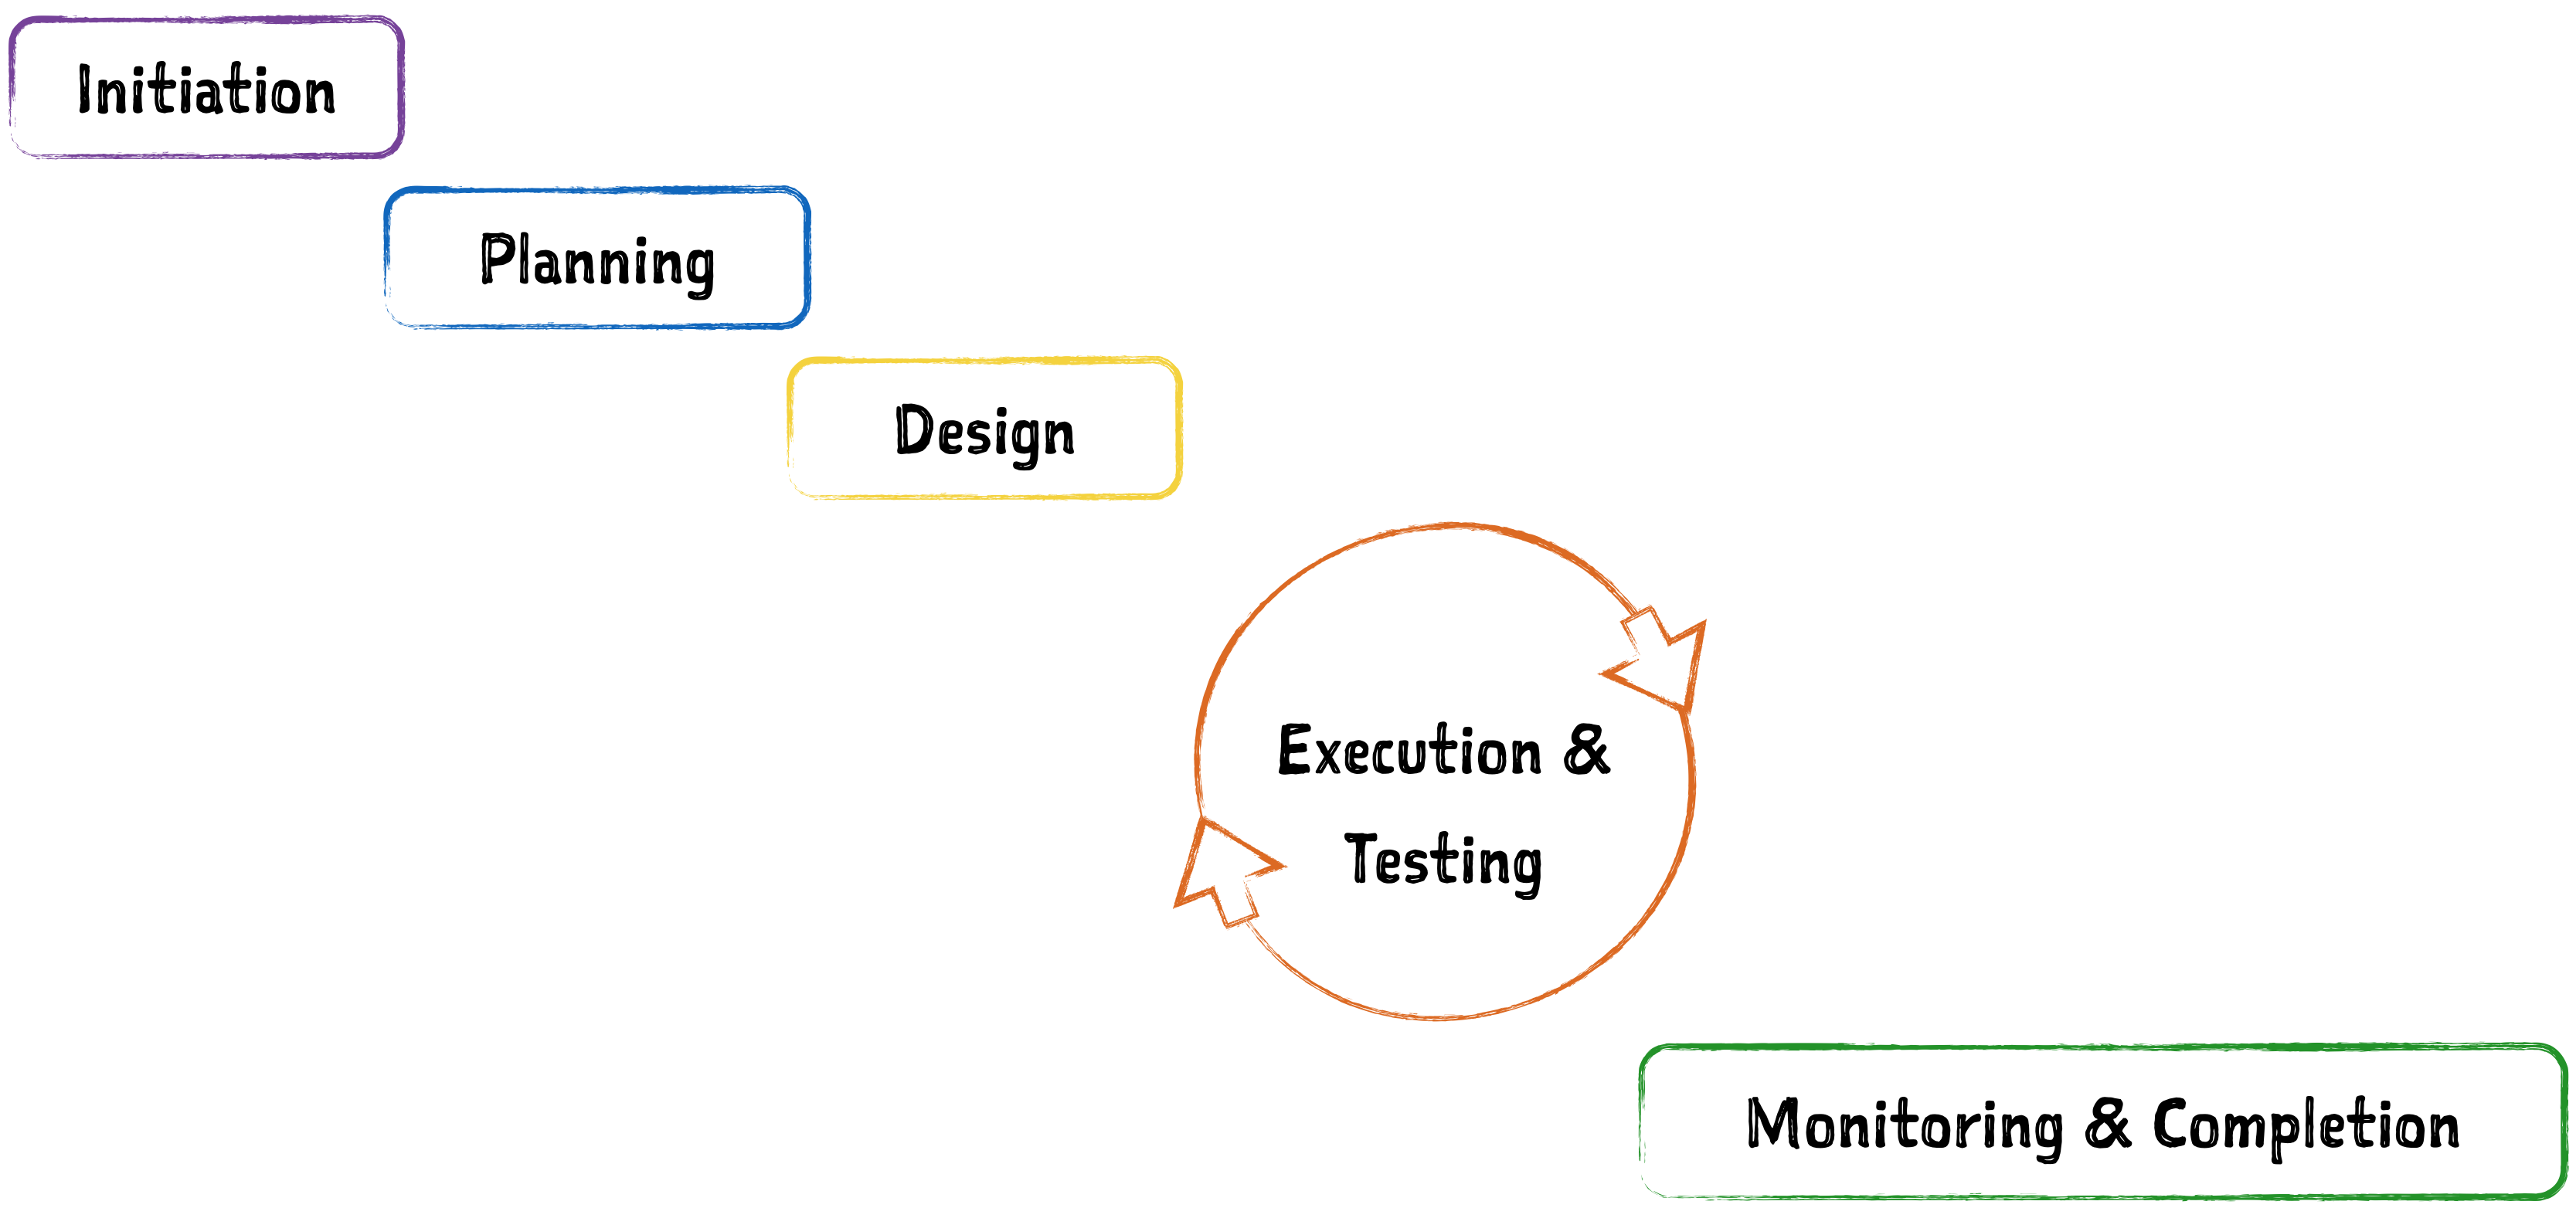
\includegraphics[scale=0.25]{proj_phases}
	\caption{مسیر پروژه}
	\label{phases} % Unique label used for referencing the figure in-text
	%\addcontentsline{toc}{figure}{Figure \ref{fig:placeholder}} % Uncomment to add the figure to the table of contents
\end{figure}

\pagebreak
\section{تحویل‌دادنی‌ها}
تحویل‌دادنی‌های هر فاز از پروژه به‌صورت زیر خواهد بود:

\begin{itemize}
	\item 
	فاز صفر
	\subitem
	پیشنهادنامه‌ی پروژه
	\item 
	فاز اول
	\subitem نمودار مورد استفاده \LTRfootnote{Use Case}
	\subitem سناریوهای سیستم
	
	\item 
	فاز دوم
	\subitem نمودار جریان داده‌ها \LTRfootnote{Data flow Diagram}
	(مدل‌سازی فرآیندها)
	\subitem
	نمودار داده رابطه‌ای
	(مدل‌سازی بانک‌های اطلاعاتی)
	\subitem معماری سیستم
	
	\item فاز سوم (پیاده‌سازی نهایی و تبدیل نمودارهای فوق به یک سیستم اطلاعاتی با استفاده از متدلوژی چابک اسکرام)
	\subitem نسخه‌ی نهایی «شریف‌کار»
	\subitem مستندات پروژه
	
\end{itemize}